\chapter{Domain Name System}
\label{cha:domain-name-system}

\section{Contact}
\label{sec:dns-contact}

\begin{table}[!h]
  \centering
  \begin{tabular}[!h]{c}
    \toprule{}
    HU Zhan \\
    zhan.hu@chinacache.com \\
    \bottomrule
  \end{tabular}
  \caption{Contact}
\end{table}

\section{Outline}
\label{sec:dns-outline}

The system resolves a \textit{fully qualified domain name} (FQDN)
of a host to IP and mainly comprises:

\begin{itemize}
\item A distributed and decentralized \textit{database}
  implemented in a hierarchy of \textit{name servers}.
\item An application layer protocol over UDP port 53, which is
  utilized by other application layer protocols like HTTP. TCP 53
  is widely supported nowadays.
\item The name servers are often UNIX machines running the
  Berkeley Internet Name Domain (BIND) or Dnsmasq software.
\item Work in Client-Server mode.
\end{itemize}

Roles:

\begin{itemize}
\item Domain: administration sapce.
\item Domain Name: name of administration space.
\item Domain · Name Servers: implement DNS database and resolve subdomain names.
\end{itemize}

\section{Domain Tree}
\label{sec:domain-tree}

\begin{figure}[tbp]
  \centering
  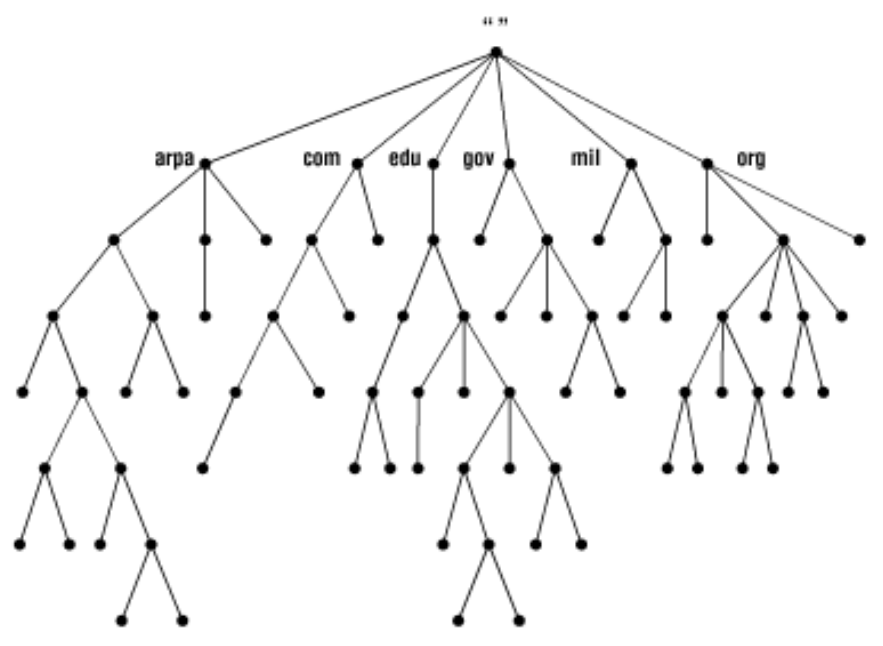
\includegraphics[scale=0.40]{domain-tree}
  \caption{Domain Tree}
  \label{fig:domain-tree}
\end{figure}

Domains define \textit{administration space} of different levels
and sizes, and can be demonstrated in a \textit{tree} structure as
depicted in figure \ref{fig:domain-tree}. External nodes
represents physical \textit{host}s. Nodes in the tree is assigned
labels, like \textit{com}, \textit{cn}, etc. A \textit{null}
\verb|""| label is reserved for the \textit{root}. But in text it
is written as a \textit{dot}. Host nodes are labelled by
\textit{hostname}s \ref{sec:dns-host}. We will find, later in the
post, each \textit{administration entity} is resposible for
managing \textit{name resolution} in its own space.

A node and the corresponding subtree represents a domain. The root
represents the whole space in DNS, namely \textit{root
  domain}. Each domain can be further divided into additional
partitions, called \textit{subdomain}s. For example, node
\textit{edu} defines a subdomain of the root domain. Domains at
the second and third layers are called \textit{Top-level Domain}
(TLD) and \textit{Authorative Domain} respectivelly.

We assign a \textit{name} to each domain, namely \textit{domain
  name}. Domain name is the sequence of labels from the
\uline{domain node} (root node of the subtree) to the
\uline{root}, with \verb|.| separating the labels. In this post,
\textit{root node} refers to that of a subtree, while
\textit{root} refers to that of the whole tree.

For instance, \textit{root domain name} is written as a dot
\uline{<.>} while \uline{<com.>} is an instance of \textit{TLD
  name}. \textit{bing.com.} is an \textit{Authorative Domain
  Name}. Attention plese; theere is one and only one root domain
name! The concepts can be illustrated as below:

\begin{quotation}
  node => subtree => domain/subdomains => domain name
\end{quotation}

DNS requires that sibling nodes have different labels to guarantee
\textit{uniquness} of domain names. Figure
\ref{fig:domain-name-uniqueness}, has two sibling nodes with
\textit{hobbes} label. That is not acceptable.

\begin{figure}
  \centering
  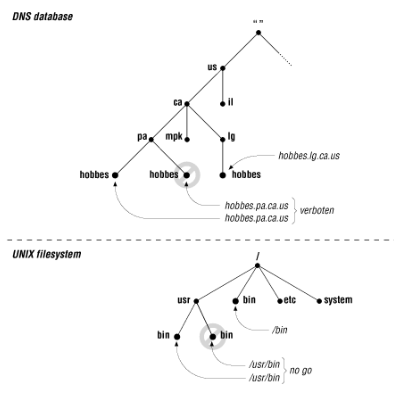
\includegraphics[scale=0.80]{domain-name-uniqueness}
  \caption{Domain Name Uniqueness}
  \label{fig:domain-name-uniqueness}
\end{figure}

The relation between domain and domain name is interesting. We can
say a domain has a domain name. We can also say a domain contains
a bunch of subdomain names. For example, a TLD named as
\textit{edu.} contains all subdomain names ending with
\textit{edu.} like \textit{berkeley.edu.} and \textit{ustc.edu.}.

Each host has domain name as well. Domain name of a host is
associated with information like IP address, name aliases, mail
routings etc. in the database. It is the original intention of DNS
to record and resolve the information associations.

Domain tree resembles the organization of an UNIX filesystem - a
database of directories and files, namely pathnames. Pathname is
analogous to domain: internal domain and directory pair, external
domain (host) and file pair are analogous. A slight difference is
the name order. In UNIX filesystem, a pathname is written in a
top-down manner while a domain name in \textit{reverse} order -
upward to the root.

\section{FQDN}
\label{sec:fqdn}

Domain name can be either \textit{absolute} or
\textit{relative}. When a domain name ends with the root label
(dot), it is an absolute domain name and also called \uline{Fully
  Qualified Domain Name} (FQDN). The root label is different from
the dot separator, though they looks the same. All domains
discussed in the prior section are absolute. Relative domain names
provided to server side will be transformed to absolute versions
by appending
\href{http://www.zytrax.com/books/dns/ch8/origin.html}{current
  ORIGIN}. The partial transformation may be done in the client
side by \textit{resolver} (check section \ref{sec:dns-resolver}).

An absolute domain name resembles an absolute pathname in UNIX
filesystem - relative to the root. A relative domain name
resembles a relative pathname - relative to the root node of a
subtree.

A relative domain name like \verb|cs.blogger| without trailing
dot, can be anywhere in the tree and may correspond to one or more
subdomains and subtrees as in figure
\ref{fig:relative-domain-name} . Analogously, multiple relative
pathnames with the same name are allowed.

\begin{figure}
  \centering
  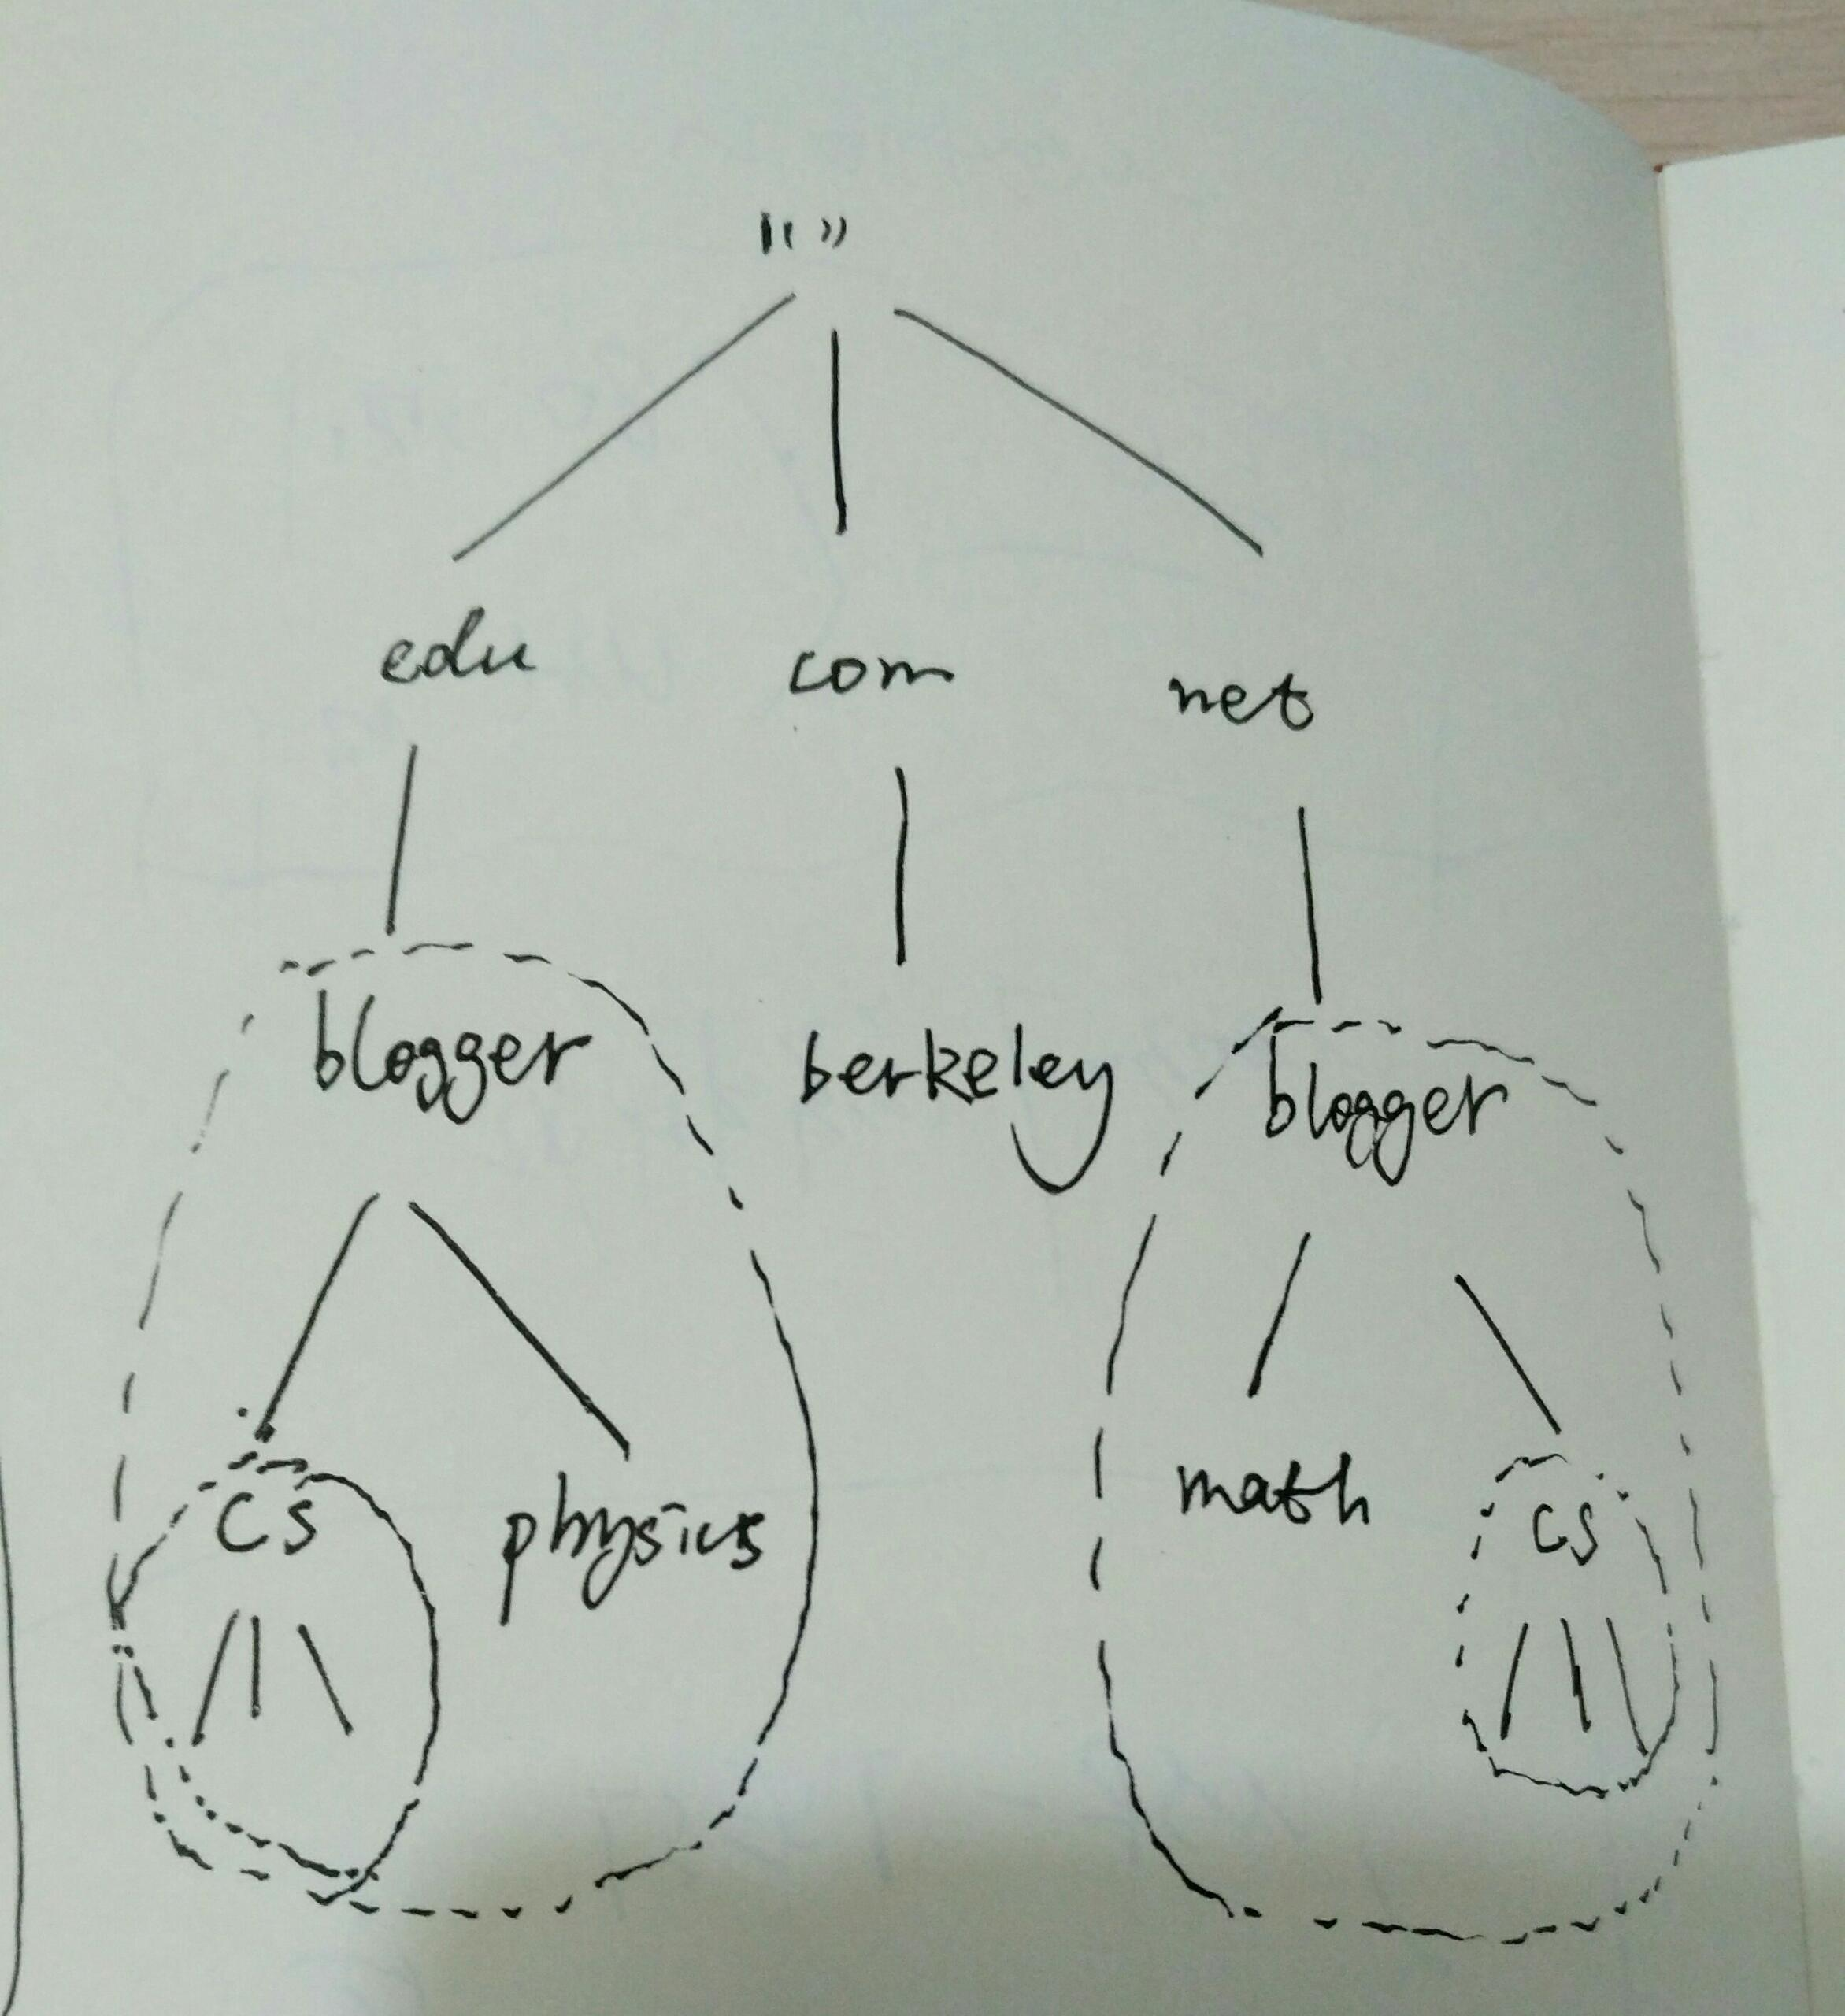
\includegraphics[scale=0.10]{relative-domain-name}
  \caption{Relative Domain Name}
  \label{fig:relative-domain-name}
\end{figure}

With respect to DNS, we'd better use FQDN as much as possible to
rid confusion.

\begin{quotation}
  Without explicit note, all domain names are \textit{absolute} in
  this post.
\end{quotation}

\section{Host}
\label{sec:dns-host}

As analyzed above, each \textit{host} has a domain name that is
also a FQDN (easy to remember by humans). Alternatively, a host
can also identified by its IP address (used by routers). FQDN of a
host can be divided into two parts, namely hostname - the first
segment, and authorative domain name - the rest part, demonstrated
in table \ref{tab:host-fqdn}:

\begin{table}[t]
  \centering
  \begin{tabular}{*{4}{|c}|}
    \hline
    www & google & com & . \\ \hline
    \multicolumn{4}{|c|}{FQDN} \\ \hline
    & \multicolumn{3}{c|}{Authorative Domain Name} \\ \hline
    && \multicolumn{2}{c|}{TLD} \\ \hline
    &&& Dot Root Domain \\ \hline
    www & google & com & . \\
    \hline
  \end{tabular}
  \caption{Host FQDN}
  \label{tab:host-fqdn}
\end{table}

\textit{hostname} in the context of DNS is different from that of
command \lstinline[language=bash]|hostname|. Instead, it is an
identfier meaningful to DNS. In the target host, both value are
not necessarily identical.

Take \textit{www.example.com.} for example, \textit{www} is the
hostname, while \textit{example.com.} is the authorative domain
name. Both names together constitute the host's FQDN.

FQDNs we use daily are actually aliases of their
\textit{canonical} versions and are far more mnemonic. A canonical
FQDN may have multiple aliases. For example,
\textit{cn-0001.cn-msedge.net.} has two aliases, one of which is
\textit{www.bing.com.}.

\begin{lstlisting}
; dig +nocookie www.bing.com cname

;; ANSWER SECTION:
www.bing.com.		60	IN	CNAME	cn.cn-0001.cn-msedge.net.
cn.cn-0001.cn-msedge.net. 36	IN	CNAME	cn-0001.cn-msedge.net.
\end{lstlisting}

About the \lstinline|dig| command, refer to section
\ref{sec:bash-dig}.

\section{Name Server}
\label{sec:domain-name-server}

How the DNS database is implemented? How domain names are
resolved? Such questions lead to the topic in this section -
\textit{domain · name server} \footnote{域 · 名字服务器}.

As mentioned in section \ref{sec:domain-tree}, an administration
entity manages domains and subdomains of its own space. An entity
can further delegates administration of subdomains to other
organizations. A domain is administrated by one and only one
entity. To the contratry, an entity can administrate one or more
domains. The core functionality of domain administration is to
implement domain · name servers and database therein,
like domain names, IPs, aliases. The entity should resolve names
of all subdomain under its coverage directly or delegate the
resolution to a sub-entity.

At the very top, we have \textit{root domain · name server}s
\footnote{根域 · 名字服务器}, then \textit{TLD · name server}s
\footnote{顶级域 · 名字服务器} at next layer, and
\textit{authorative domain · name server}s \footnote{权威域 · 名字
  服务器}. Root domain name servers are responsible to resolve TLD
names while TLD name servers are for authorative domain
names. Authorative domain name servers resolve host FQDNs instead.

\section{Resource Record}
\label{sec:resource-record}

Now let's have a closer insight into what DNS database looks
like. We call a DNS entry in the database Resource Record
(RR). The relationship line can be put like below:

\begin{quotation}
  doname name => administration space => administration entity =>
  domain name · servers =>
  database => subdomain RRs => subdomains resolution \\
\end{quotation}

RRs are indexed by domain names in DNS database. The snippet
\ref{lst:dns-database-index} are excerpts from one of the root
domain name servers. Each entry is queried by TLD name
\verb|<com.>|.

\begin{lstlisting}[caption={DNS Database Index},label={lst:dns-database-index}]
com.			172800	IN	NS	a.gtld-servers.net.
com.			172800	IN	NS	b.gtld-servers.net.
com.			172800	IN	NS	c.gtld-servers.net.
com.			172800	IN	NS	l.gtld-servers.net.
com.			172800	IN	NS	m.gtld-servers.net.
\end{lstlisting}

There exist multiple types of RRs like SOA, PTR etc. But they are
not the core of the post. Here are four common types of RRs as
follows:

\begin{itemize}
\item A: (domain name, ip)
\item NS: (domain name, domain name server)
\item CNAME: (alias, canonical domain name)
\item MX: (mail domain name, alias)
\end{itemize}

If a domain name server contains an A record for a particular
subdomain name, it is \textit{authorative} for that name. Needless
to say, it is an authorative domain name server. If a domain name
server contains an SOA record, it is also authorative (check
section \ref{sec:zone-data-file}). In this post, authorative
domain name server only refers to those resolving host FQDNs.

Most the of RRs in a name server are NS records that specify
alternative domain name servers (at a lower level \footnote{A NS
  RR reflects the delegation of administration.}) from which the
subdomain name can be resolved. It is sensible that internal FQDNs
require only NS records as they just do auxiliary jobs for
resolving external FQDNs (that of hosts).

Those alternative domain name servers, in return, are all physical
hosts in the system and should have their own external
FQDNs. Accordingly, there \textit{must} exist A records somewhere
in the system. In other words, the selected external FQDN should
be resolved first before the original query. This process may
repeat several times during the resolution course.

\section{Root Domain Name Server}
\label{sec:root-domain-name-server}

There are overall 13 root domain name servers over the world,
namely \lstinline[language=bash]|{a..m}.root-servers-net.|. The
relevant 13 IP addresses are fixed and kept by all name servers in
the system, such that there is no need to resolve root domain
name. This makes sure the resolving system starts with an initial
entrance.

Those 13 name servers are authorative for TLD names
(i.e. \uline{<com.>} and \uline{<net.>}) and contain NS records,
pointing where TLD names can be resolved. From excerpt
\ref{lst:root-ns-rr}, the root domain name server
\textit{b.root-servers.net.} contain 13 \footnote{The number of
  TLD name server is also 13.} NS records the TLD name
\textit{com.}.

\begin{minipage}{1.0\linewidth}
\begin{lstlisting}[caption={RRs in Root Name Server},label={lst:root-ns-rr},basicstyle=\tiny\ttfamily]
; <<>> DiG 9.11.2-P1 <<>> +trace www.bing.com
;; global options: +cmd
.			82248	IN	NS	d.root-servers.net.
.			82248	IN	NS	k.root-servers.net.
.			82248	IN	NS	c.root-servers.net.
.			82248	IN	NS	e.root-servers.net.
.			82248	IN	NS	b.root-servers.net.
.			82248	IN	NS	j.root-servers.net.
.			82248	IN	NS	h.root-servers.net.
.			82248	IN	NS	i.root-servers.net.
.			82248	IN	NS	f.root-servers.net.
.			82248	IN	NS	m.root-servers.net.
.			82248	IN	NS	g.root-servers.net.
.			82248	IN	NS	l.root-servers.net.
.			82248	IN	NS	a.root-servers.net.
;; Received 736 bytes from 127.0.0.1#53(127.0.0.1) in 2 ms

com.			172800	IN	NS	d.gtld-servers.net.
com.			172800	IN	NS	c.gtld-servers.net.
com.			172800	IN	NS	i.gtld-servers.net.
com.			172800	IN	NS	j.gtld-servers.net.
com.			172800	IN	NS	l.gtld-servers.net.
com.			172800	IN	NS	f.gtld-servers.net.
com.			172800	IN	NS	a.gtld-servers.net.
com.			172800	IN	NS	g.gtld-servers.net.
com.			172800	IN	NS	h.gtld-servers.net.
com.			172800	IN	NS	e.gtld-servers.net.
com.			172800	IN	NS	m.gtld-servers.net.
com.			172800	IN	NS	b.gtld-servers.net.
com.			172800	IN	NS	k.gtld-servers.net.
;; Received 1172 bytes from 199.9.14.201#53(b.root-servers.net) in 198 ms
\end{lstlisting}
\end{minipage}

Specially, root name servers are authorative for each other and
should contain A records as in excerpt \ref{lst:root-a-rr}. The
root name server \textit{j.root-servers.net.} are authorative for
\textit{a.root-servers.net.} .

\begin{minipage}{1.0\linewidth}
\begin{lstlisting}[caption={A RR in Root Name Server},label={lst:root-a-rr},basicstyle=\tiny\ttfamily]
a.root-servers.net.	3600000	IN	A	198.41.0.4
root-servers.net.	3600000	IN	NS	a.root-servers.net.
root-servers.net.	3600000	IN	NS	b.root-servers.net.
root-servers.net.	3600000	IN	NS	c.root-servers.net.
root-servers.net.	3600000	IN	NS	d.root-servers.net.
root-servers.net.	3600000	IN	NS	e.root-servers.net.
root-servers.net.	3600000	IN	NS	f.root-servers.net.
root-servers.net.	3600000	IN	NS	g.root-servers.net.
root-servers.net.	3600000	IN	NS	h.root-servers.net.
root-servers.net.	3600000	IN	NS	i.root-servers.net.
root-servers.net.	3600000	IN	NS	j.root-servers.net.
root-servers.net.	3600000	IN	NS	k.root-servers.net.
root-servers.net.	3600000	IN	NS	l.root-servers.net.
root-servers.net.	3600000	IN	NS	m.root-servers.net.
;; Received 825 bytes from 192.58.128.30#53(j.root-servers.net) in 3 ms
\end{lstlisting}
\end{minipage}

\section{DNS Query}
\label{sec:dns-query}

The resolution process goes in the reverse direction than FQDN. A
FQDN is scanned from right to left along the tree in a top-down
approach. Query is sent to a \textit{local default name server}
first and then routed hierarchically.

A local name server commonly is given by ISP and acts as a DNS
proxy for all its customers. Though it does not belong to the DNS
hierarchy, a local name server is critical to DNS resolution.

Local name servers send customers' queries to the a root domain
name server first, and then repeat \textit{iteratively} or
\textit{recursively} through the system.

Iterative method means each DNS reply is sent back directly to the
original query client and new queries are sent out
accordingly. Resursive queries \ref{fig:recursive-dns-queries}
mean each name server along the path acts as a DNS proxy and
forwards the query on behalf of the preceding client and returns A
records to it.

In reality, the resolution process may combine both methods. In
figure \ref{fig:itera-recur-quer-dns}, request from
\textit{cis.poly.edu.} to \textit{dns.poly.edu.} belongs to
recursive query while those from \textit{dns.poly.edu} to all
other upstream name servers belong to interative queries.

\begin{figure}[tbp]
  \centering
  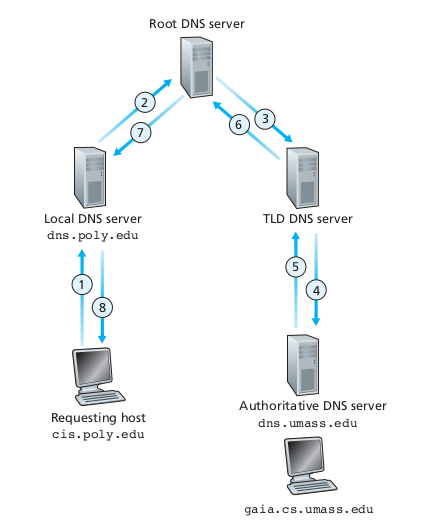
\includegraphics[scale=0.50]{recursiveDNSQueries}
  \caption{Recursive queries in DNS}
  \label{fig:recursive-dns-queries}
\end{figure}

\begin{figure}[tbp]
  \centering
  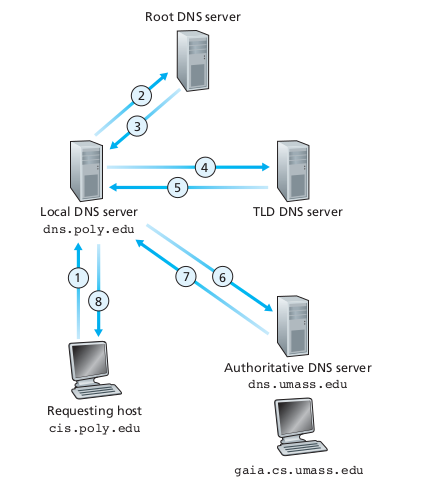
\includegraphics[scale=.50]{recurIteraDNSQueries}
  \caption{Iterative and recursive queries in DNS}
  \label{fig:itera-recur-quer-dns}
\end{figure}

\section{DNS Cache}
\label{sec:dns-cache}

Upon receving authorative results from upper level, a name server
chooses to \textbf{cache} the mapping results for a fixed period
(the 2nd column of \lstinline|dig| output), within which, new
matched queries are served immediately. DNS caching can manifestly
reduce DNS resolution time and improve user experience.

Although a domain name can be resolved by different domain name
servers with DNS cache, those servers must have an authorative
source (check SOA in section \ref{sec:zone-data-file}).

\section{Round Robin}
\label{sec:dns-round-robin}

Round Robin is a technique of load distribution/balancing,
provisioning multiple and redundant service hosts by managing DNS
responses to address queries.

Most network application have a list of backend hosts and IPs
thereof. The order of IPs returned are permuted in a round robin
way.

Generally, a client application just pick the very first IP from
the reply, so that different clients would receive service from
different backends, thus distributing the overall load among
servers.

\section{Anycast}
\label{sec:dns-anycast}

Apart from Round Robin, the system also adopts
\href{https://en.wikipedia.org/wiki/Anycast}{Anycast} to eliminate
the bottleneck of 13 root name servers. Name server IP has a bunch
of backend hosts.

With the help of BGP routing and Automation System (AS), DNS
queries are distrubted to a geographically nearby host.

\section{Zone Data File}
\label{sec:zone-data-file}

RRs are actually defined in \textit{zone data file}s of name
servers. As mentioned, a domain name server cannot have all the
records of the whole database. A zone data file contains only part
of the complete database. The term zone is analogous to domain,
but not identical. For example, a zone data file may contain only
part of RRs for a domain.

Basically, there are two types of zone data file. One is in the
form of \uline{db.DOMAIN} that maps domain names to IPs, which is
called \textit{forward mapping}. Take domain name
\textit{bing.com} for example, forward mapping records are stored
in file \textit{db.bing.com}.

The other type is for \uline{reverse mapping} that maps IPs to
domain names in the form of \uline{db.ADDR}, where \uline{ADDR} is
the network address without trailing zeros. Take block
\textit{192.249.249.0/24} for example, its zone data file is
\textit{db.192.249.249}. Records in this type are called
\href{https://en.wikipedia.org/wiki/Reverse_DNS_lookup}{PTR}.

Zone data files are also called \textit{db} files. Any DNS
implementation (i.e. BIND and Dnsmasq) must have these zone data
files to support lookups. Also, they must comply with the same
data format - \uline{master file format}
\ref{sec:master-file-format}.

How these files are organized and located depends on
\uline{connfiguration file}. For BIND 8 or 9, the configuration
file is \textit{/etc/named.conf}. The format of configuration file
is flexible and depends on implementations.

\section{Master File Format}
\label{sec:master-file-format}

Text after semicolon to the end of a line is treated as
comments. Code \verb|$TTL| set the cache time of a record.

Start of Authority (SOA) record is a must for every domain name
server, indicating this server is the \textit{best} source of
information for the data within this zone. There can be one and
only one SOA record in each a data zone file.

Here is an excerpt of a SOA query for
\textit{www.bing.com.}. Obviously, db files on servers
\textit{ns1.cn-msedge.net.} and \textit{msnhst.microsoft.com.}
should contain such SOA record.

\begin{lstlisting}
; dig www.bing.com soa
cn-msedge.net.		59	IN	SOA	ns1.cn-msedge.net. msnhst.microsoft.com. 2017032701 1800 900 2419200 240
\end{lstlisting}

SOA record is also used to do zone data file
\href{https://en.wikipedia.org/wiki/DNS_zone_transfer}{synchronization}
periodically among distributed domain name servers in the
system. Ideally, each server should cache as many RRs as
possible. However, it is infeasible as the size is too much to
hold and the increased synchronization traffic is beyond
negligibleness.

Pointer (PTR) record accomplishes reverse mapping. The firstly
field is a concatanation of a reverse network address and suffix
domain \textit{in-addr.arpa}. PTR records must point to
\textit{canonical} domain names instead of aliases:

\begin{lstlisting}
; dig -x 204.79.197.200
200.197.79.204.in-addr.arpa. 2806 IN	PTR	a-0001.a-msedge.net.
\end{lstlisting}

In a \uline{db.domain} file, symbol \verb|@| can be used to
replace current ORIGIN. For example, a MX record \ref{lst:mx-rr}
usually starts with \verb|@|:

\begin{minipage}{1.0\linewidth}
\begin{lstlisting}[caption={MX RR},label={lst:mx-rr}]
# db.movie.edu
@ IN SOA terminator.movie.edu. al.robocop.movie.edu. (
                          1h   ; serial number
                          3h   ; refresh after 3 hours
                          1h   ; retry after 1 hour
                          1w   ; expire after 1 week
                          1h ) ; negative expiration
\end{lstlisting}
\end{minipage}

\section{Resolver}
\label{sec:dns-resolver}

Once DNS is implemented, how to make use of it? We need
\textit{resolver}. Resolvers are the clients that access name
servers when any programs running need name resolution.

Resolvers require configuration (\verb|/etc/resolv.conf|)
beforehand and allow customization of the following items:

\begin{itemize}
\item default \textit{domain} directive;
\item \textit{search} list directive;
\item \textit{nameserver}s directive;
\item \textit{sortlist} directive;
\item \textit{optoin}s directive.
\end{itemize}

The \textit{domain} and \textit{search} directives are mainly used
to make users' lives easier by saving them some typing. Both
directives generate a list of relative domain names. When domain
names sent to the resolver are relative (not FQDN), it would
prepend the input to the each relative domain name in the
list. The resulted domain names sent to namer servers is still
relative, and will be appended by current ORIGIN.

%%% Local Variables:
%%% mode: latex
%%% TeX-master: "main"
%%% End:
